\subsection{V4: изменение структуры твэла}

Расчет V4 проверяет не увеличение мощности в прежнем твэле, а изменение пути теплопередачи. Топливо заменено расчетным кольцевым высокотеплопроводным керметным слоем \(r=3.40\text{--}4.00\,\mathrm{мм}\). Между активным слоем и оболочкой оставлен почти связанный контакт \(h_g=10^6\,\mathrm{Вт/(м^2\,K)}\), а W-оболочка уменьшена до \(0.195\,\mathrm{мм}\). Энергия по-прежнему вводится только в топливо GeN-Foam; отдельного нагревателя пара нет.

\begin{figure}[H]
    \centering
    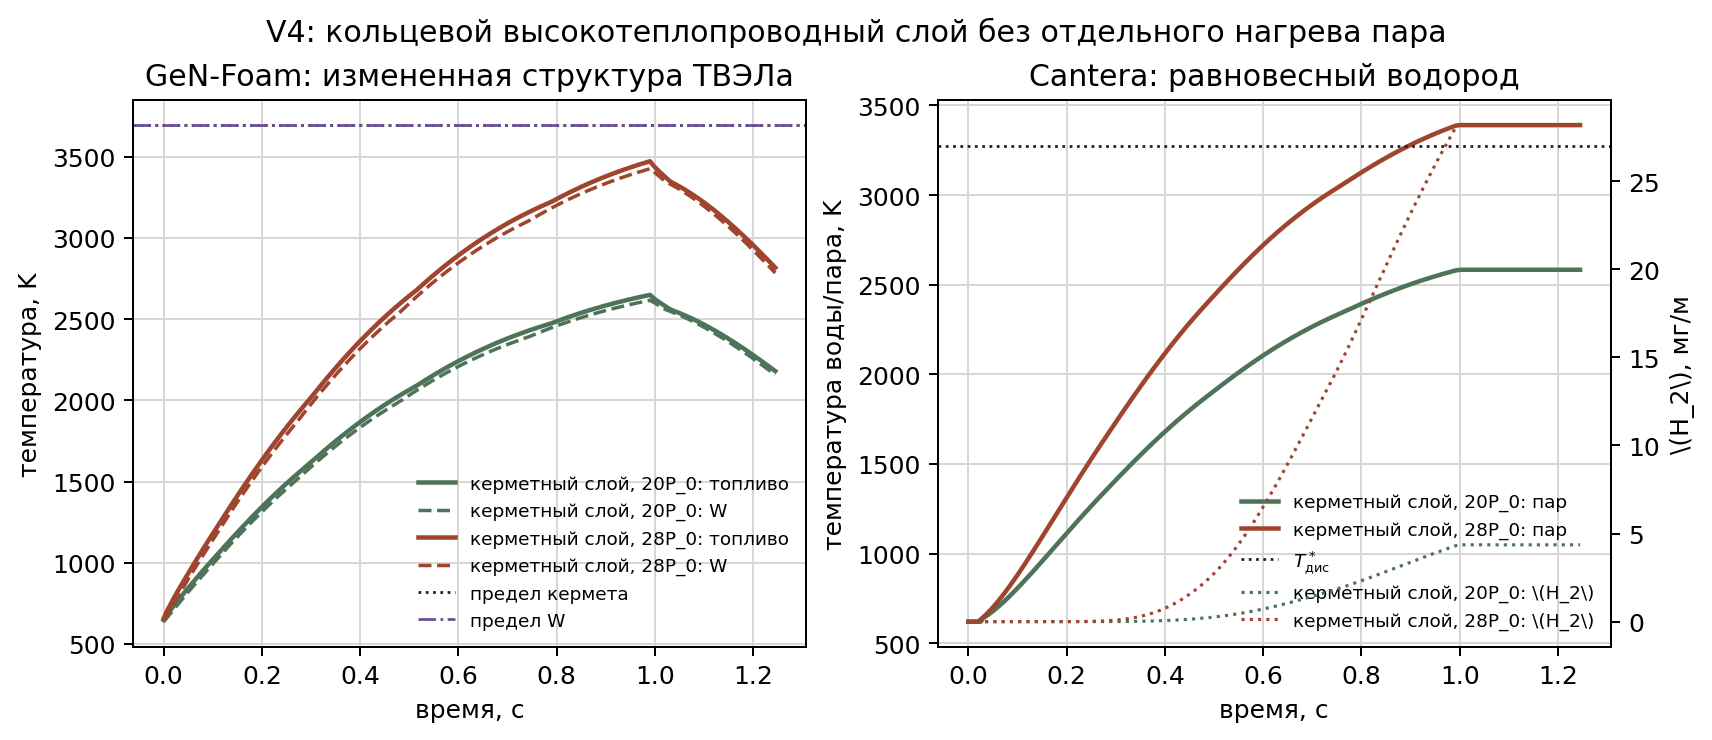
\includegraphics[width=0.88\textwidth]{figures/pipeline_v4_structured_tvel.png}
    \caption{V4: кольцевой высокотеплопроводный слой снижает радиальный перегрев топлива и позволяет наружной W-стенке открыть температурное окно для воды/пара. Cantera дает равновесную оценку \(H_2\), а не извлекаемую массу продукта.}
    \label{fig:pipelineV4StructuredTvel}
\end{figure}

\begin{table}[H]
    \centering
    \caption{Проверка измененной структуры твэла: нагрев только через топливо.}
    \label{tab:pipelineV4StructuredTvel}
    \footnotesize
    \resizebox{\textwidth}{!}{%
    \begin{tabular}{@{}p{3.7cm}rrrrrrp{5.1cm}@{}}
    \hline
    Сценарий & \(P/P_0\) & \(T_f^{\max}\), K & \(T_W^{\max}\), K & \(T_s^{\max}\), K & \(E'_w\), кДж/м & \(m_{H_2}\), мг/м & Вывод \\
    \hline
    керметный слой, \(20P_0\) & 20 & 2650 & 2616 & 2583 & 21.79 & 4.36 & пределы соблюдены, но окно не открыто \\
керметный слой, \(28P_0\) & 28 & 3473 & 3426 & 3391 & 29.16 & 28.18 & кандидатный режим: паровое окно достигнуто без перегрева \\
    \hline
    \end{tabular}
    }
\end{table}

Положительный расчетный режим возникает только после изменения геометрии теплопередачи. При \(20P_0\) структура остается холоднее пределов, но пар не достигает \(T^*_{\mathrm{дис}}\). При \(28P_0\) максимум пара составляет около \(3390\,\mathrm{K}\), максимум топлива около \(3470\,\mathrm{K}\), а W-оболочки около \(3430\,\mathrm{K}\). Эти значения ниже принятого теплового предела \(3695\,\mathrm{K}\), поэтому в рамках текущей тепловой модели появляется кандидатный режим образования \(H_2\). Он не является проектом реактора: керметный слой, W-стенка в паре, механика тонкой оболочки, нейтроника, радиационная граница и химическая кинетика требуют отдельной квалификации.
